% Chapter 4: Release 2 (End-to-End Encrypted Communication and P2P)

\chapter{Release 2}
\label{ch:chapter4}

\section{Introduction}
This chapter details the conceptualization, design, and implementation of Release 2, which constitutes the most critical phase of our project by establishing its core security and privacy features. This release is divided into three highly specialized sprints: Sprint 3 focuses on securing text communications through robust AES-256-GCM encryption, Sprint 4 is dedicated to engineering a secure Peer-to-Peer (P2P) WebRTC voice calling architecture that bypasses centralized media servers, and Sprint 5 ensures transparency and usability through open-source self-hosting capabilities and extended UI features. For each sprint, we outline the product backlog, analyze the dynamic and static system designs using UML modeling, and conclude by demonstrating the implemented functionalities that validate our rigorous security requirements.

\section{Sprint 3}

\subsection{Sprint 3 Overview}
The objective of this sprint is to establish real-time encrypted messaging and instant chat history delivery. The user stories allocated to this sprint are described in Table~\ref{tab:sprint3_backlog}.


\renewcommand{\arraystretch}{1.5}
\begin{longtable}{| p{1.4cm} | p{10cm} | p{2.0cm} | p{1.5cm} |}
    \hline
    \rowcolor{lightgray}
    \textbf{ID} & \textbf{User Story \& Acceptance Criteria} & \textbf{Priority} & \textbf{Points} \\
    \hline
    \endfirsthead
    \hline
    \rowcolor{lightgray}
    \textbf{ID} & \textbf{User Story \& Acceptance Criteria} & \textbf{Priority} & \textbf{Points} \\
    \hline
    \endhead
    \hline
    \endfoot
    \hline
    \endlastfoot
\renewcommand{\arraystretch}{1.0} % Reset spacing for the rest of the document

    S3-01 & \textbf{As a} server member, \textbf{I want to} send a message in a text channel and have everyone see it instantly, \textbf{so that} we can have a real-time conversation.
    \newline \textit{Acceptance Criteria}:
    \newline \textbullet\ Messages appear for all members of the channel without refreshing.
    \newline \textbullet\ Message includes my name and the time it was sent.
    \newline \textbullet\ An empty message cannot be sent. & P0 & 8 \\
    \hline
    S3-02 & \textbf{As a} server member, \textbf{I want to} see recent messages when I open a channel, \textbf{so that} I can catch up on what was discussed before I arrived.
    \newline \textit{Acceptance Criteria}:
    \newline \textbullet\ The last 50 messages load when I open a channel.
    \newline \textbullet\ Messages are shown in chronological order.
    \newline \textbullet\ Each message shows the sender's name and timestamp. & P1 & 3 \\
    \hline
    S3-03 & \textbf{As a} server member, \textbf{I want to} see which members of a server are online or offline, \textbf{so that} I know who is available to chat.
    \newline \textit{Acceptance Criteria}:
    \newline \textbullet\ Online members are visually distinct from offline ones.
    \newline \textbullet\ My status becomes online when I log in.
    \newline \textbullet\ My status becomes offline when I close the app. & P1 & 3 \\
    \hline
    S3-04 & \textbf{As a} server member, \textbf{I want to} edit my own messages after sending them, \textbf{so that} I can fix mistakes.
    \newline \textit{Acceptance Criteria}:
    \newline \textbullet\ I can edit the text of a message I sent.
    \newline \textbullet\ The message shows an 'edited' label.
    \newline \textbullet\ Other members cannot edit my messages. & P1 & 2 \\
    \hline
    S3-05 & \textbf{As a} server member, \textbf{I want to} delete my own messages, \textbf{so that} I can remove something I no longer want to have posted.
    \newline \textit{Acceptance Criteria}:
    \newline \textbullet\ My message disappears for all members.
 \newline \textbullet\ I can only delete my own messages unless I have a moderation role.
    \newline \textbullet\ Deletion is immediate and cannot be undone. & P1 & 2 \\
    \hline
    \caption{\textbf{Sprint 3 Backlog - Real-Time Chat \& Presence.}}
    \label{tab:sprint3_backlog}
\end{longtable}
\normalsize

\subsection{Designing the Static View}
The static view of a system focuses on its structural aspects, such as the entities it manages and the relationships among them.

\subsubsection{Use Case Diagram}
The following diagram highlights the core interactions introduced in this sprint, specifically focusing on the sending of messages and related functionalities.

\begin{figure}[H]
    \centering
    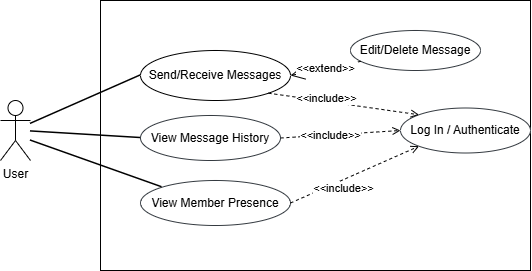
\includegraphics[width=0.9\textwidth]{UseCaseGeneral-send_message_sprint3.png}
    \caption{Use Case Diagram: Sending a Message (Sprint 3).}
    \label{fig:usecase_sprint3}
\end{figure}


\subsection{Cryptographic Algorithm Selection}

When designing the encryption pipeline to guarantee the confidentiality and integrity of messages at rest, several cryptographic algorithms were evaluated. Table~\ref{tab:crypto_comparison} outlines the comparison between the considered options:

\renewcommand{\arraystretch}{1.15}
\begin{table}[H]
    \centering
    \small
    \begin{tabular}{| p{3cm} | p{2.2cm} | p{2.8cm} | p{6.5cm} |}
        \hline
        \rowcolor{lightgray}
        \textbf{Algorithm} & \textbf{Type} & \textbf{Integrity Check} & \textbf{Drawbacks / Fit} \\
        \hline
        \textbf{AES-256-GCM} & Symmetric (AEAD) & Built-in (Auth Tag) & Hardware accelerated (AES-NI), extremely fast, and provides built-in tampering protection. \\
        \hline
        \textbf{AES-256-CBC} & Symmetric Block & None (Requires HMAC) & Requires padding; vulnerable to padding oracle attacks without strict MAC implementations. \\
        \hline
        \textbf{ChaCha20-Poly1305} & Symmetric (AEAD) & Built-in (Poly1305) & Excellent for mobile/software environments, but AES-GCM performs faster on modern servers with AES-NI. \\
        \hline
        \textbf{RSA-4096} & Asymmetric & Depends on scheme & Computationally prohibitive for real-time bulk message encryption; only suited for key exchanges. \\
        \hline
    \end{tabular}
    \vspace{0.2cm}
    \caption{Comparison of encryption algorithms.}
    \label{tab:crypto_comparison}
\end{table}
\renewcommand{\arraystretch}{1.0}

\paragraph{Algorithm Choice and Justification:}
Based on this analysis, \textbf{AES-256-GCM} (Advanced Encryption Standard with a 256-bit key in Galois/Counter Mode) was selected as the optimal choice for our platform. It strikes the perfect balance between robust security, built-in integrity validation, and high throughput leveraging CPU hardware acceleration, which is critical for a real-time messaging server processing massive amounts of chat data.

\paragraph{Algorithm Overview:}
AES-256-GCM is an industry-standard symmetric-key block cipher that provides Authenticated Encryption with Associated Data (AEAD). This means it simultaneously guarantees data confidentiality and authenticity (integrity). The Galois field multiplication used in the counter mode generates an authentication tag that ensures the encrypted ciphertext has not been tampered with.

\subsection{Designing the Dynamic View}
The dynamic perspective shows how software system elements interact and act together with a focus on action sequences and message passing among them.

\paragraph{AES-256-GCM Encryption Pipeline:}
Before a message is stored, it passes through the encryption service layer:
\begin{itemize}
    \item The plaintext message payload is passed to the \texttt{MessageCryptoService}.
    \item The service encrypts the content using AES-256-GCM with a server-managed secret key loaded from the environment configuration.
    \item The resulting base64-encoded ciphertext is persisted to the database; no plaintext is ever written.
\end{itemize}

\subsubsection{Design Sequence Diagram}
We illustrate here the operation flow and transition among the various layers of an application through design sequence diagrams in this section.

\begin{itemize}
\item \textbf{Design Sequence Diagram: "Sending a Message with Encryption"}
\end{itemize}
The diagram below details the server-side AES-256-GCM encryption flow when a message is sent:

\begin{figure}[H]
    \centering
    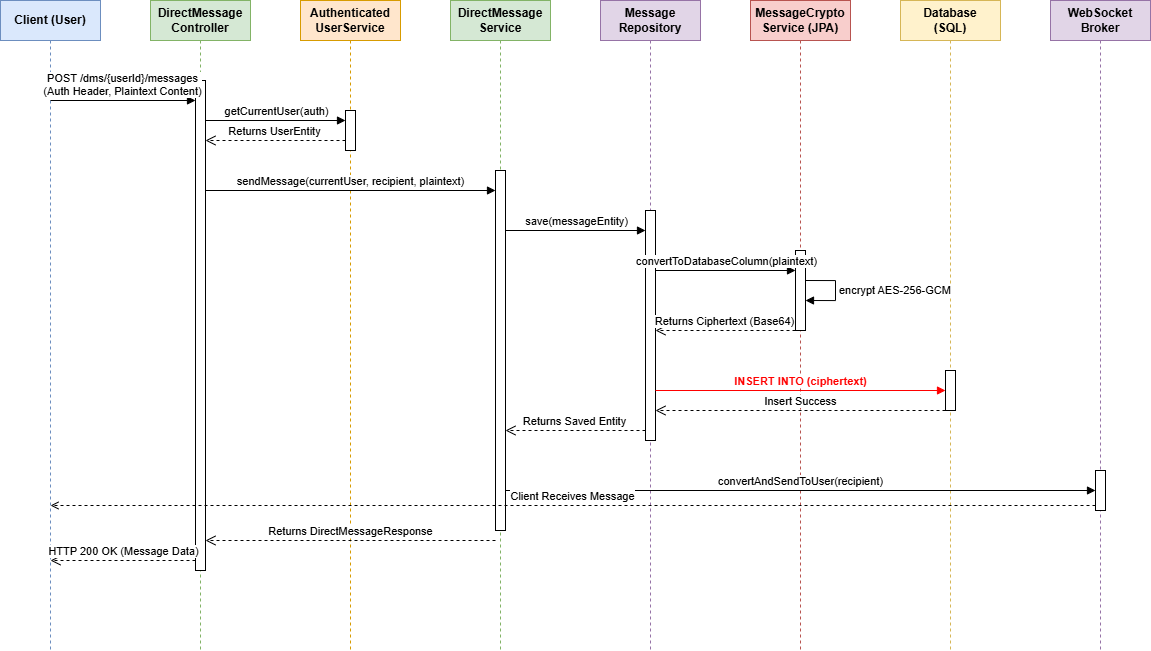
\includegraphics[width=1\textwidth]{seq_diag_enc_sptint2.drawio.png}
    \caption{Sequence Diagram: Sending a Message with Encryption.}
    \label{fig:sprint3_seq_enc}
\end{figure}

\subsubsection{State Transition Diagram}
A state transition diagram illustrates the different states an entity can be in during its lifecycle and how it transitions from one state to another based on specific events or conditions. The diagram below shows the various statuses a user's presence can have within the platform (e.g., Online, Offline, Idle, Do Not Disturb). 

\vspace{0.2cm}
\noindent\colorbox{lightgray}{%
    \parbox{\dimexpr\textwidth-2\fboxsep\relax}{%
        \textbf{Note:} Users have the ability to manually change their presence state at any time to appear in whatever state they wish, overriding automatic transitions.
    }%
}
\vspace{0.2cm}

\begin{figure}[H]
    \centering
    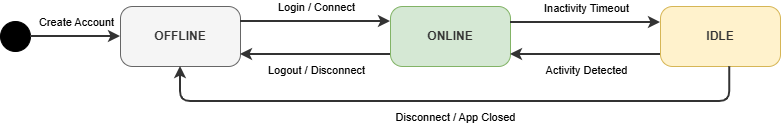
\includegraphics[width=0.8\textwidth]{sprint2_state_diag.drawio.png}
    \caption{State Transition Diagram for User Presence.}
    \label{fig:sprint3_state_diag}
\end{figure}




\subsection{Class Diagram}
The class diagram below illustrates the internal structure of the messaging module and the relationships between users, messages, and channels.

\begin{figure}[H]
    \centering
    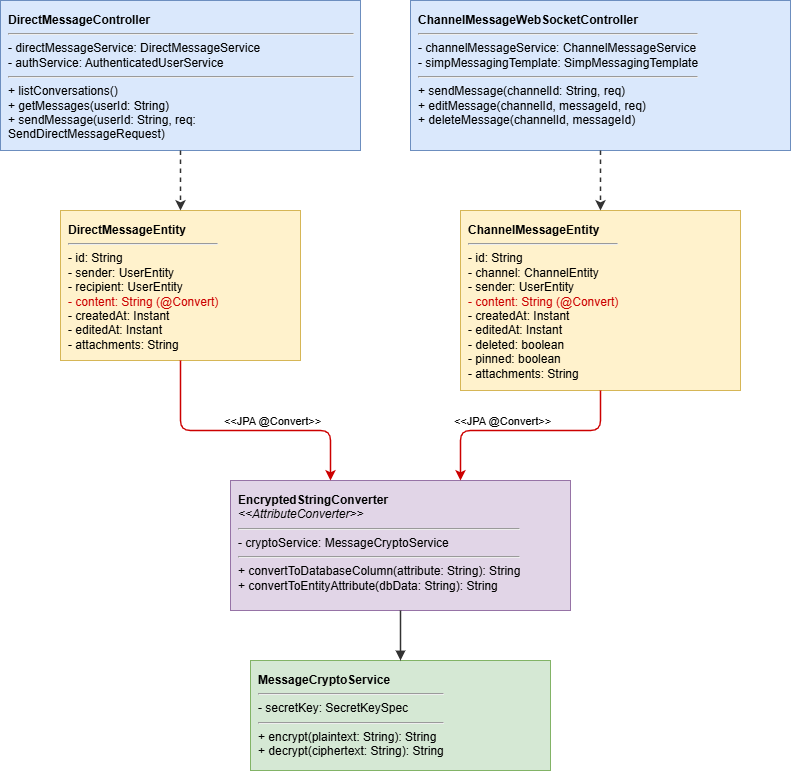
\includegraphics[width=0.8\textwidth]{class_diag_sprint3.png}
    \caption{Class Diagram for Real-Time Chat (Sprint 3).}
    \label{fig:class_sprint3}
\end{figure}
\vspace{0.2cm}
\noindent\colorbox{lightgray}{%
    \parbox{\dimexpr\textwidth-2\fboxsep\relax}{%
        \textbf{Note:} The \texttt{@Convert} annotation leverages \texttt{EncryptedStringConverter} to intercept all database operations. This provides transparent, ``Zero-Knowledge'' AES-256-GCM encryption at the lowest boundary, automatically encrypting data on save and decrypting on load so application services can safely work with plaintext.
    }%
}
\vspace{0.2cm}


\subsection{Sprint 3 Review}
During the Sprint Review, the team presented:
\begin{itemize}
    \item \textbf{Client Chat Interface}: Messages are rendered dynamically inside the browser window for all users in the channel.
    \item \textbf{Database Persistence Proof}: A capture of the SQL database console, proving that the server only stores unreadable ciphertexts (e.g. \code{content = "eyJhY2N1cm9...=="}), confirming successful AES-256-GCM encryption at rest.
    \textbf{Direct Messaging and Friends System}: Validated the ability to list conversations, send direct messages, and manage friend requests (sending, handling duplicates, and accepting).
\end{itemize}

% --- AUDIT SCREENSHOTS (Sprint 3) ---

\begin{figure}[H]
    \centering
    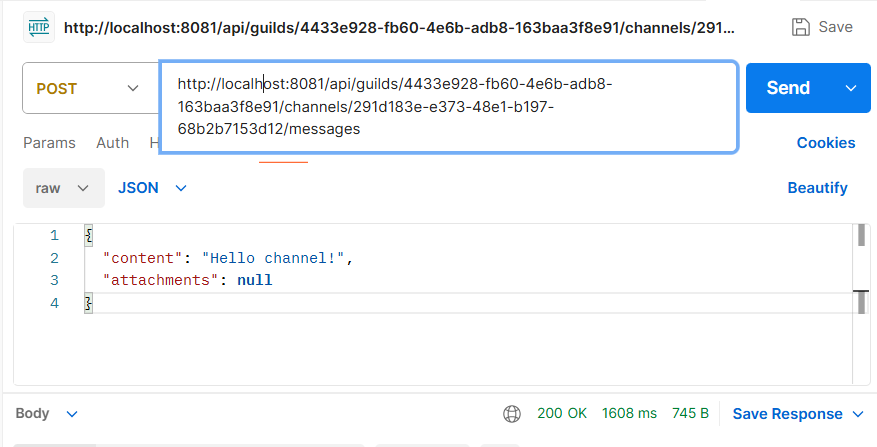
\includegraphics[width=0.7\textwidth]{send message in text channel.png}
    \caption{Audit: Sending Messages in a Server Channel.}
    \label{fig:sprint3_send_msg}
\end{figure}

\begin{figure}[H]
    \centering
    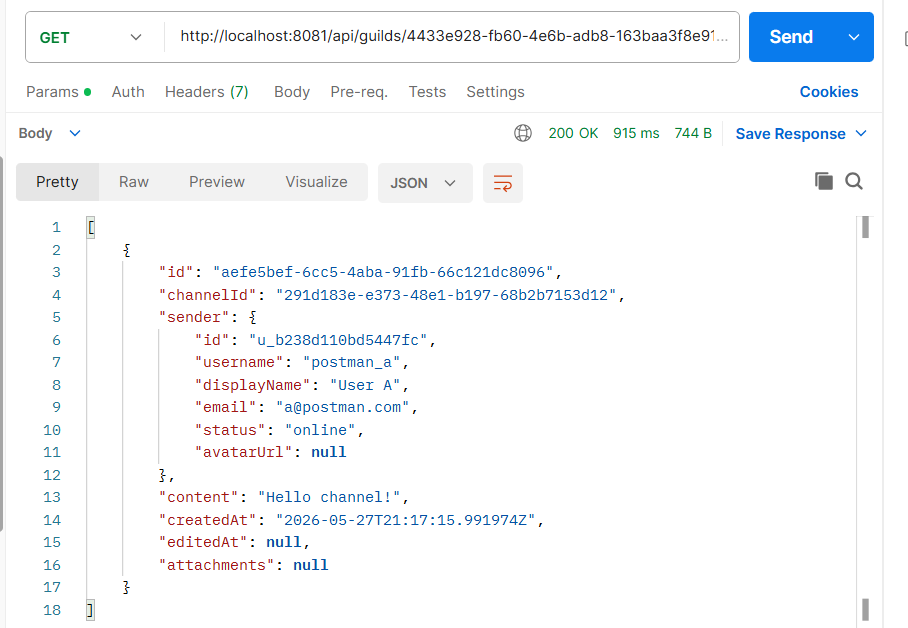
\includegraphics[width=0.7\textwidth]{fetch messages in channels.png}
    \caption{Audit: Fetching Message History.}
    \label{fig:sprint3_fetch_msg}
\end{figure}

\begin{figure}[H]
    \centering
    % Filename has a space, wrapped in braces
    \includegraphics[width=0.7\textwidth]{{list conversation .png}}
    \caption{Audit: Listing Direct Message Conversations.}
    \label{fig:sprint3_dm_list}
\end{figure}

\begin{figure}[H]
    % Filename has a space, wrapped in braces
    \includegraphics[width=0.7\textwidth]{{send dm .png}}
    \caption{Audit: Sending a Direct Message.}
    \label{fig:sprint3_send_dm}
\end{figure}

\begin{figure}[H]
    \centering
    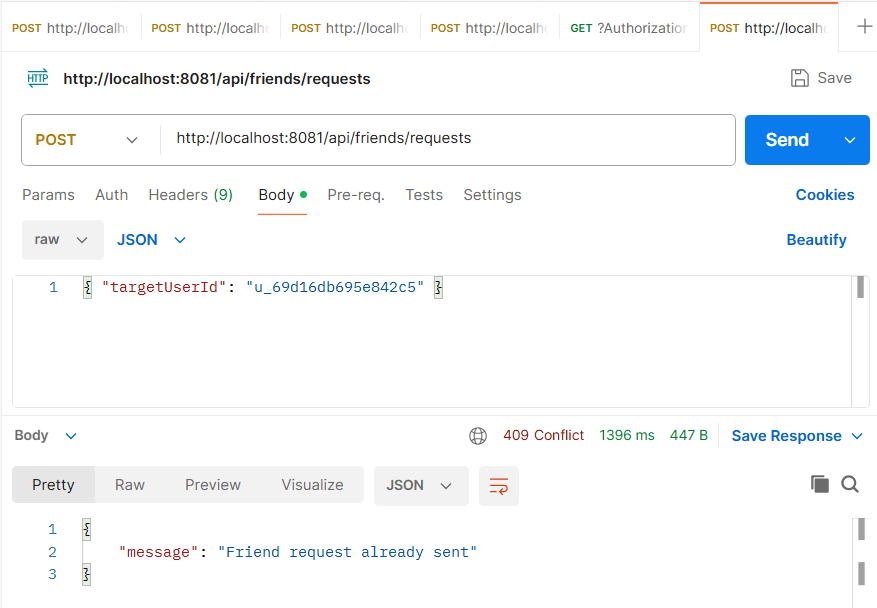
\includegraphics[width=0.7\textwidth]{friend request already sent.png}
    \caption{Audit: Handling Duplicate Friend Requests.}
    \label{fig:sprint3_friend_dup}
\end{figure}

\begin{figure}[H]
    \centering
    % Filename has parentheses
    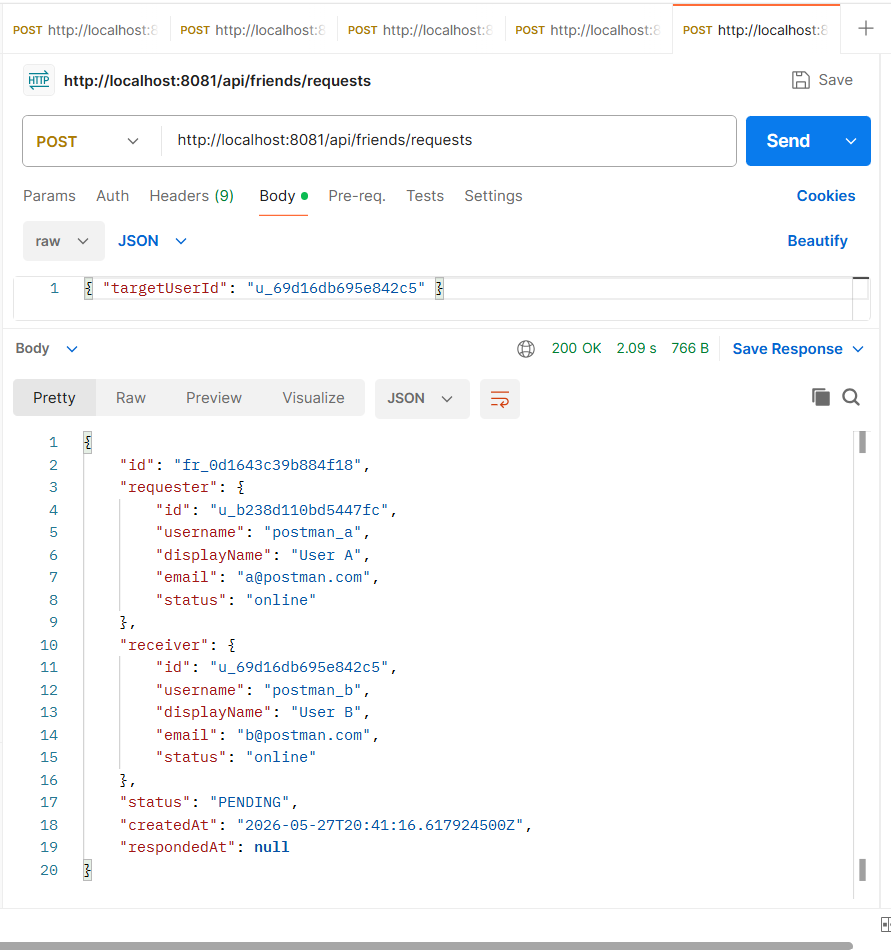
\includegraphics[width=0.7\textwidth]{friendrequest (send).png}
    \caption{Audit: Sending a Friend Request.}
    \label{fig:sprint3_friend_send}
\end{figure}

\begin{figure}[H]
    % Note: Filename has typo "freind" -> "friend" in the filename, keeping it as provided
    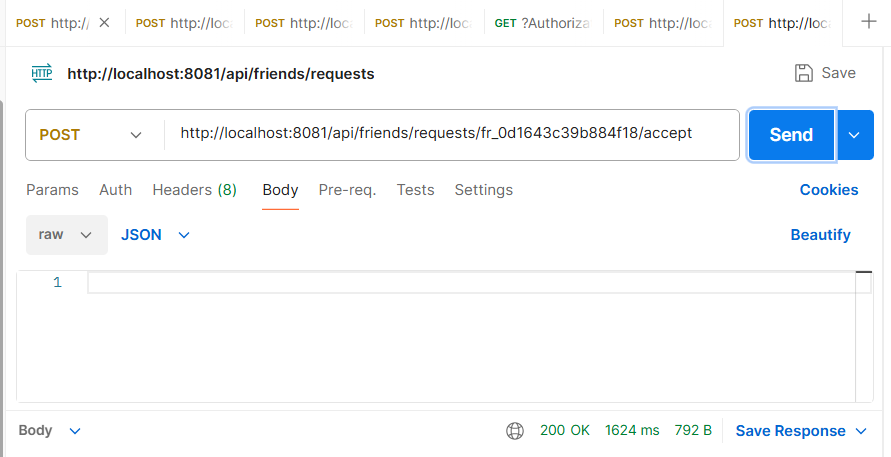
\includegraphics[width=0.7\textwidth]{accept freind request.png}
    \caption{Audit: Accepting a Friend Request.}
    \label{fig:sprint3_friend_accept}
\end{figure}

\subsection{Sprint 3 Retrospective}
The AES-256-GCM encryption layer introduced no noticeable latency for end users. The team noted that since messages are encrypted at rest, any full-text search functionality must be implemented at the application layer after decryption, rather than delegated to the database engine. Additionally, while the current implementation utilizes a server-managed secret key for encryption, a future migration to a fully decentralized client-side key generation model is planned to achieve the strict Zero-Knowledge architecture outlined in the project objectives.

\section{Sprint 4: Secure Peer-to-Peer (P2P) Voice Calls}
Sprint 4 implements direct, secure real-time audio rooms.

\subsection{Sprint 4 Overview}
The goal of this sprint is to bypass centralized media servers. Active participant audio streams flow directly IP-to-IP using WebRTC. The central server is used solely as a neutral signaling relay (SDP/ICE candidate exchange), and direct streams are secured against wiretapping via DTLS/SRTP.

\subsection{Sprint 4 Backlog}
The primary objective of \textbf{Sprint 4} is to establish secure P2P voice call channels. The user stories allocated to this sprint are described in Table~\ref{tab:sprint4_backlog}.

    
\renewcommand{\arraystretch}{1.5}
\begin{longtable}{| p{1.4cm} | p{10cm} | p{2.0cm} | p{1.5cm} |}
    \hline
    \rowcolor{lightgray}
    \textbf{ID} & \textbf{User Story \& Acceptance Criteria} & \textbf{Priority} & \textbf{Points} \\
    \hline
    \endfirsthead
    \hline
    \rowcolor{lightgray}
    \textbf{ID} & \textbf{User Story \& Acceptance Criteria} & \textbf{Priority} & \textbf{Points} \\
    \hline
    \endhead
    \hline
    \endfoot
    \hline
    \endlastfoot
\renewcommand{\arraystretch}{1.0} % Reset spacing for the rest of the document

    S4-01 & \textbf{As a} server member, \textbf{I want to} join a voice channel and talk with others in real time, \textbf{so that} we can have live voice conversations.
    \newline \textit{Acceptance Criteria}:
    \newline \textbullet\ I can join a voice channel and hear other members.
    \newline \textbullet\ Other members can hear me.
    \newline \textbullet\ I appear in the voice channel participant list when connected. & P0 & 8 \\
    \hline
    S4-02 & \textbf{As a} voice channel participant, \textbf{I want to} mute my microphone, \textbf{so that} I can stop broadcasting audio without leaving the channel.
    \newline \textit{Acceptance Criteria}:
    \newline \textbullet\ Muting stops my audio from being heard by others.
    \newline \textbullet\ Other members see that I am muted.
    \newline \textbullet\ I can unmute myself at any time. & P1 & 2 \\
    \hline
    S4-03 & \textbf{As a} voice channel participant, \textbf{I want to} deafen myself, \textbf{so that} I can stop hearing others without leaving the channel.
    \newline \textit{Acceptance Criteria}:
    \newline \textbullet\ Deafening stops all incoming audio.
    \newline \textbullet\ Other members see that I am deafened.
    \newline \textbullet\ I can un-deafen myself at any time. & P1 & 2 \\
    \hline
    S4-04 & \textbf{As a} voice channel participant, \textbf{I want to} see who is currently in the voice channel, \textbf{so that} I can follow the conversation and know who is present.
    \newline \textit{Acceptance Criteria}:
    \newline \textbullet\ A list of participants in the voice channel is visible.
    \newline \textbullet\ The list updates in real time as people join or leave. & P1 & 3 \\
    \hline
    S4-05 & \textbf{As a} voice channel participant, \textbf{I want to} leave the voice channel, \textbf{so that} I stop being part of the voice call.
    \newline \textit{Acceptance Criteria}:
    \newline \textbullet\ Leaving removes me from the participant list.
    \newline \textbullet\ Other members are notified that I left.
    \newline \textbullet\ My audio is no longer broadcast. & P1 & 1 \\
    \hline
    \caption{\textbf{Sprint 4 Backlog - Peer-to-Peer Voice Engine.}}
    \label{tab:sprint4_backlog}
\end{longtable}
\normalsize

\subsection{Designing the Static View}
The static view of a system focuses on its structural aspects, such as the entities it manages and the relationships among them.

\subsubsection{Use Case Diagram}
The following diagram highlights the core interactions introduced in this sprint, specifically focusing on the initiation and management of voice channels.

\begin{figure}[H]
    \centering
    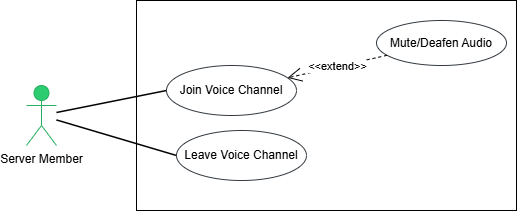
\includegraphics[width=0.9\textwidth]{UseCase_sprint4.png}
    \caption{Use Case Diagram: Voice Channels (Sprint 4).}
    \label{fig:usecase_sprint4}
\end{figure}

\subsection{Designing the Dynamic View}
The dynamic perspective shows how software system elements interact and act together with a focus on action sequences and message passing among them.

\subsubsection*{State Transition Diagram}
\paragraph{WebRTC Connection Lifecycle Explanation:}
The state transition diagram illustrates the lifecycle of the \texttt{RTCPeerConnection} during real-time voice communication. Initially, the connection starts in an \textbf{Idle} state. Upon initiating a call, the system transitions to the \textbf{Signaling / Negotiating} state, where Session Description Protocol (SDP) offers and answers are exchanged through the STOMP WebSocket signaling server. Once the local descriptions are set, the connection enters the \textbf{Gathering ICE Candidates} phase. During this phase, STUN servers are queried to discover the public network addresses (ICE candidates) necessary to bypass NATs and firewalls. If a valid peer-to-peer route is established and the DTLS handshake succeeds, the state transitions to \textbf{Connected}, allowing bidirectional audio streaming. The connection will transition to \textbf{Disconnected} upon user termination, or fallback to \textbf{Failed} if NAT traversal cannot establish a direct path.

\begin{figure}[H]
    \centering
    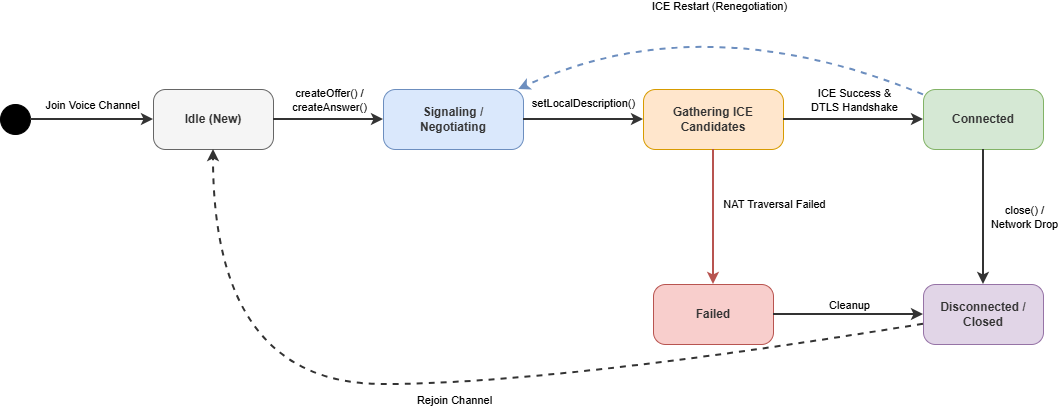
\includegraphics[width=0.9\textwidth]{sprint4_websocket_state.drawio.png}
    \caption{State Transition Diagram: WebRTC Connection Lifecycle.}
    \label{fig:sprint4_state_webrtc}
\end{figure}


\subsubsection{Design Sequence Diagram}
We illustrate here the operation flow and transition among the various layers of an application through design sequence diagrams in this section.

\begin{itemize}
\item \textbf{Design Sequence Diagram: "WebRTC Signaling Sequence"}
\end{itemize}
Here is the highly detailed Sequence Diagram illustrating how your STOMP WebSocket acts as the middleman for WebRTC Signaling (exchanging Offers, Answers, and ICE Candidates).

\begin{figure}[H]
    \centering
    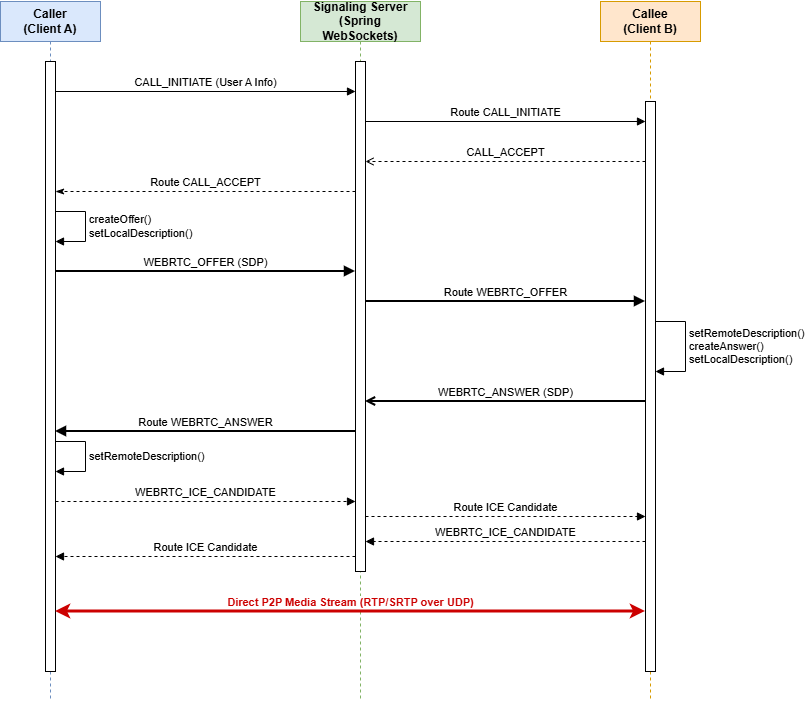
\includegraphics[width=0.9\textwidth]{sprint4_diag_seq.drawio.png}
    \caption{WebRTC Signaling Sequence Diagram.}
    \label{fig:sprint4_seq_webrtc}
\end{figure}

\subsubsection{Security Architecture: DTLS and SRTP}
WebRTC mandates encryption for all media and data streams. To achieve this, it utilizes Datagram Transport Layer Security (DTLS) and Secure Real-time Transport Protocol (SRTP). DTLS provides a secure handshake over UDP, facilitating cryptographic key exchange without the need to transmit keys through the signaling server. Once the keys are securely exchanged between peers, they are used to establish an SRTP session, which encrypts and authenticates the real-time audio (and video) streams during transit. This ensures that peer-to-peer communication is fully protected against eavesdropping and Man-in-the-Middle (MitM) attacks.

\begin{figure}[H]
    \centering
    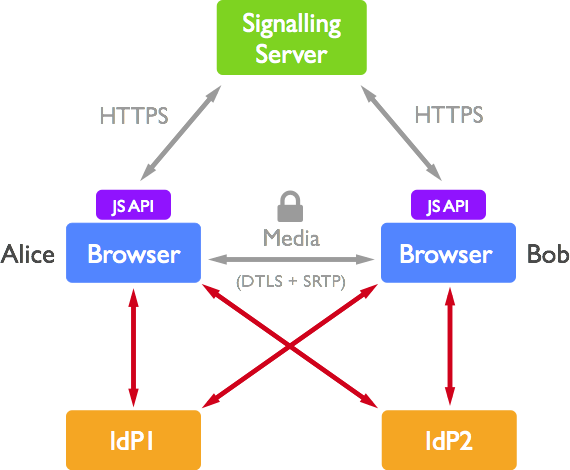
\includegraphics[width=0.8\textwidth]{diagram_4_en.png}
    \caption{DTLS-SRTP Security Architecture (Source: webrtc-security.github.io).}
    \label{fig:sprint4_dtls_srtp}
\end{figure}

\subsection{Sprint 4 Review}
The sprint review validated:
\begin{itemize}
    \item \textbf{Voice Channel Interface}: A dynamic UI featuring participant list cards and visual active-speaker borders.
    \item \textbf{Direct IP Routing Proof}: WebRTC internals and browser console captures showing audio streams transiting directly IP-to-IP, completely bypassing our backend server.
\end{itemize}

% --- AUDIT SCREENSHOTS (Sprint 4) ---

\begin{figure}[H]
    \centering
    % Filename has a space before extension, wrapped in braces
    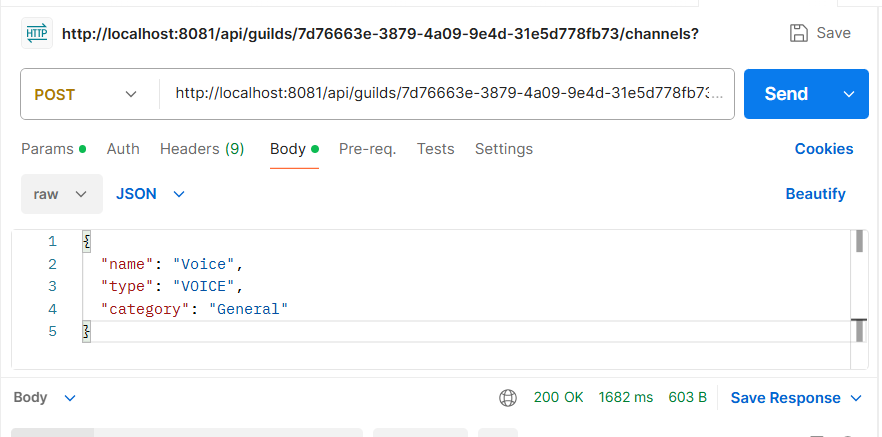
\includegraphics[width=0.7\textwidth]{voice channel creation .png}
    \caption{Audit: Creating a Voice Channel.}
    \label{fig:sprint4_review_create}
\end{figure}

\begin{figure}[H]
    \centering
    % Filename has typo "voic", kept as is
    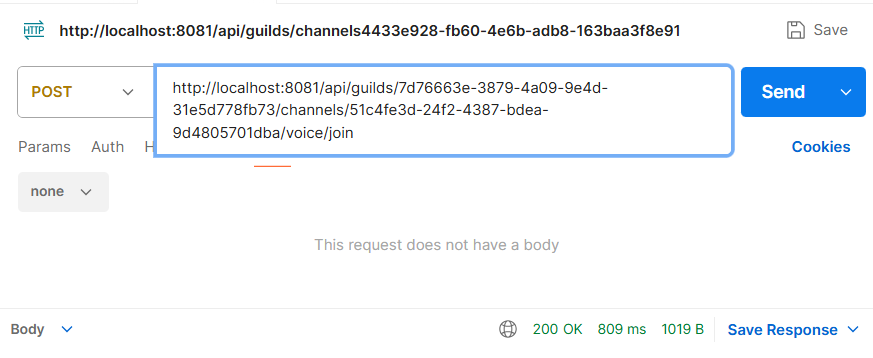
\includegraphics[width=0.7\textwidth]{join voic channel.png}
    \caption{Audit: Joining a Voice Channel.}
    \label{fig:sprint4_review_join}
\end{figure}

\begin{figure}[H]
    \centering
    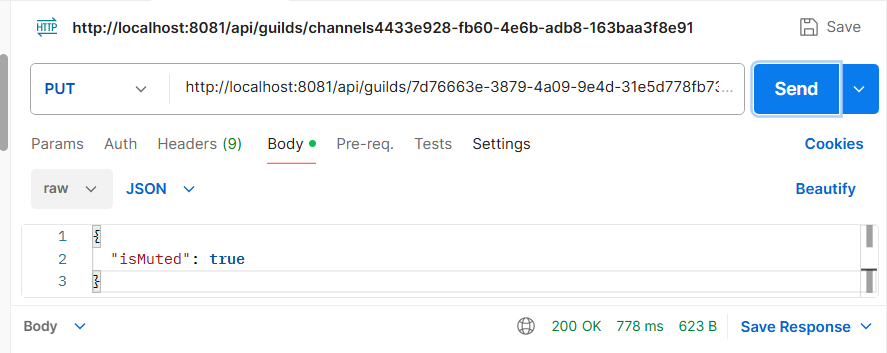
\includegraphics[width=0.7\textwidth]{mute in guild.png}
    \caption{Audit: Muting the Microphone.}
    \label{fig:sprint4_review_mute}
\end{figure}

\begin{figure}[H]
    \centering
    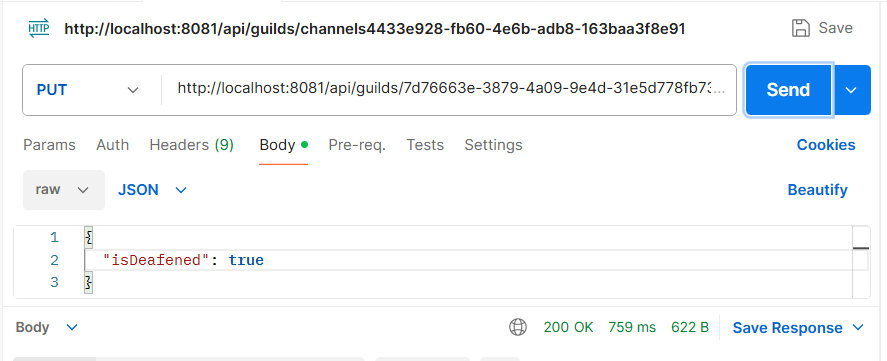
\includegraphics[width=0.7\textwidth]{deafen.png}
    \caption{Audit: Deafening Audio Output.}
    \label{fig:sprint4_review_deafen}
\end{figure}

\begin{figure}[H]
    \centering
    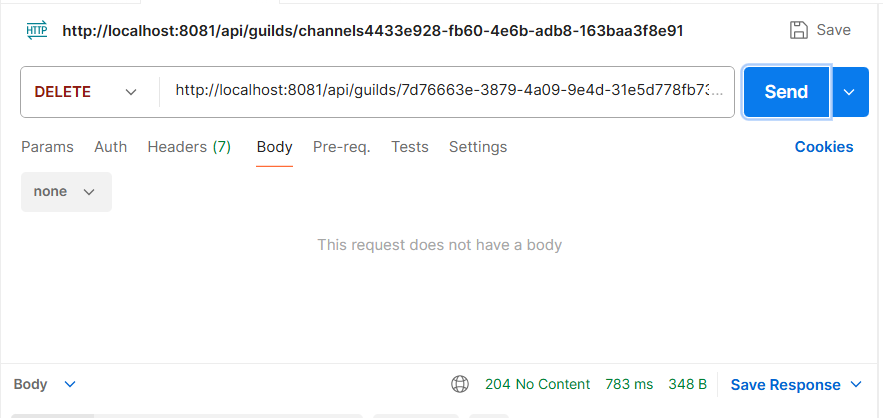
\includegraphics[width=0.7\textwidth]{leave voice channel.png}
    \caption{Audit: Leaving a Voice Channel.}
    \label{fig:sprint4_review_leave}
\end{figure}

\subsection{Sprint 4 Retrospective}
In this section, we discuss what we successfully accomplished as well as the missing elements of our sprint, presented in Table~\ref{tab:sprint4_retro}.

\renewcommand{\arraystretch}{1.5}
\begin{table}[H]
    \centering
    \begin{tabular}{| p{7.5cm} | p{7.5cm} |}
        \hline
        \textbf{Successes} & \textbf{Missing Elements} \\
        \hline
        \begin{itemize}
            \item Implemented a decentralized peer-to-peer WebRTC voice engine.
            \item Enabled secure, real-time voice channels with DTLS/SRTP encryption.
            \item Fully implemented core features: joining/leaving channels, microphone muting, and deafening.
        \end{itemize} & 
        \begin{itemize}
            \item Failed to implement visual active-speaker highlighting due to Web Audio API complexities.
            \item Connection quality degradation when participants are behind restrictive Symmetric NATs (deferred to future perspectives).
        \end{itemize} \\
        \hline
    \end{tabular}
    \caption{Successes and missing elements of Sprint 4.}
    \label{tab:sprint4_retro}
\end{table}
\renewcommand{\arraystretch}{1.0}

\section{Sprint 5: Open-Source and Auditability (Extended)}
Sprint 5 focuses on code transparency, self-hosting configurations, and client auditing.

\subsection{Sprint 5 Overview}
This sprint establishes the foundation for self-hosting and security auditing. The primary implementation effort was directed towards infrastructure: packaging the signaling server and frontend client into independent Docker containers and developing tools for cryptographic verification. Additionally, the team aimed to deliver items from the Extended Backlog, including message editing, file attachments, interface theming, and direct message notifications.

\subsection{Extended Sprint 5 Backlog}
The user stories allocated to this sprint are described in Table~\ref{tab:extended_backlog}.

    
\renewcommand{\arraystretch}{1.5}
\begin{longtable}{| p{1.4cm} | p{10cm} | p{2.0cm} | p{1.5cm} |}
    \hline
    \rowcolor{lightgray}
    \textbf{ID} & \textbf{User Story \& Acceptance Criteria} & \textbf{Priority} & \textbf{Points} \\
    \hline
    \endfirsthead
    \hline
    \rowcolor{lightgray}
    \textbf{ID} & \textbf{User Story \& Acceptance Criteria} & \textbf{Priority} & \textbf{Points} \\
    \hline
    \endhead
    \hline
    \endfoot
    \hline
    \endlastfoot
\renewcommand{\arraystretch}{1.0} % Reset spacing for the rest of the document

    EXT-01 & \textbf{As a} server member, \textbf{I want to} attach an image or a file to a message, \textbf{so that} I can share content with other members.
    \newline \textit{Acceptance Criteria}:
    \newline \textbullet\ Files up to 10 MB are accepted.
    \newline \textbullet\ The file appears in the chat.
    \newline \textbullet\ Files larger than 10 MB are rejected with a clear error. & P1 & 5 \\
    \hline
    EXT-02 & \textbf{As a} user, \textbf{I want to} switch to a dark mode interface, \textbf{so that} the app is comfortable to use at night.
    \newline \textit{Acceptance Criteria}:
    \newline \textbullet\ A toggle switches between light and dark mode.
    \newline \textbullet\ My preference is saved and remembered.
    \newline \textbullet\ All screens respect the active theme. & P2 & 2 \\
    \hline
    EXT-03 & \textbf{As a} user, \textbf{I want to} receive a notification when I am mentioned in a Direct Message, \textbf{so that} I do not miss messages addressed to me directly.
    \newline \textit{Acceptance Criteria}:
    \newline \textbullet\ A notification badge appears when I receive a Direct Message mentioning me.
    \newline \textbullet\ The badge clears when I open the conversation.
    \newline \textbullet\ Notifications are scoped to Direct Messages only. & P2 & 3 \\
    \hline
    \caption{\textbf{Extended Backlog - Sprint 5 \& Beyond.}}
    \label{tab:extended_backlog}
\end{longtable}
\normalsize

\subsection{Designing the Static View}
The static view of a system focuses on its structural aspects, such as the entities it manages and the relationships among them.

\subsubsection{Use Case Diagram}
The following diagram highlights the core interactions introduced in the extended backlog, focusing on file attachments, theming, and notifications.

\begin{figure}[H]
    \centering
    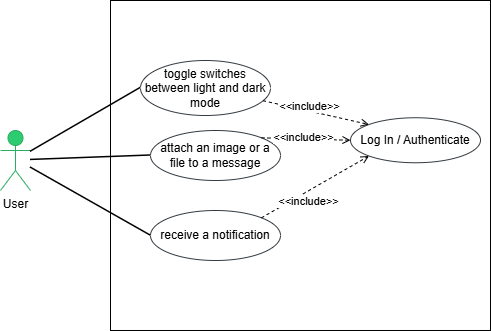
\includegraphics[width=0.9\textwidth]{UseCase_sprint 5.png}
    \caption{Use Case Diagram: Extended Features (Sprint 5).}
    \label{fig:usecase_sprint5}
\end{figure}

\subsection{Designing the Dynamic View}
The dynamic perspective shows how software system elements interact and act together with a focus on action sequences and message passing among them.

\subsubsection{Activity Diagram}
An activity diagram shows the sequence of operations and actions in a process. It allows for the modeling of a system’s process steps and decision points in each stage.

\begin{itemize}
\item \textbf{Activity Diagram: "File Upload Process"}
\end{itemize}
The activity flow below outlines the process of validating and uploading a file attachment:

\begin{figure}[H]
    \centering
    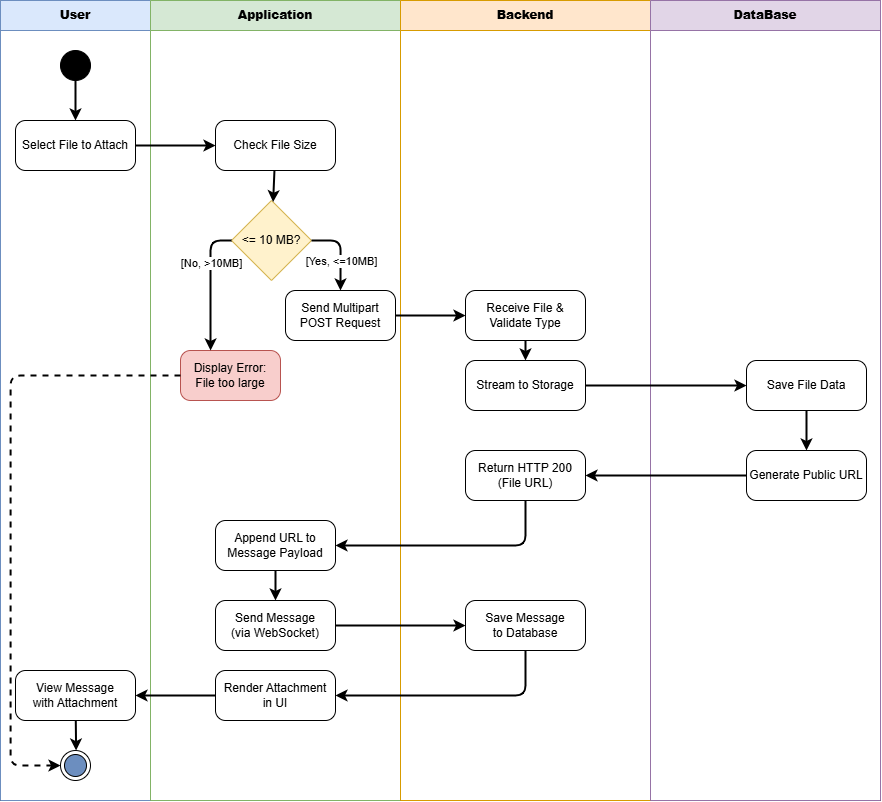
\includegraphics[width=0.9\textwidth]{sprint5_diag activity.png}
    \caption{Activity Diagram: File Upload Process.}
    \label{fig:sprint5_activity_file_upload}
\end{figure}


\subsection{Sprint 5 Review}
The sprint review validated the delivery of the Extended Backlog items and confirmed the auditability of the foundational system security:

\begin{itemize}
    \item \textbf{File Attachments}: Verified the ability to upload and display files within chat channels.
    \item \textbf{Security Audit of Foundation Modules}: Conducted validation tests on the server provisioning, role management, and permission systems (originally implemented in Sprint 2) to ensure proper access control and security.
\end{itemize}

% --- AUDIT SCREENSHOTS (Sprint 5) ---

\begin{figure}[H]
    \centering
    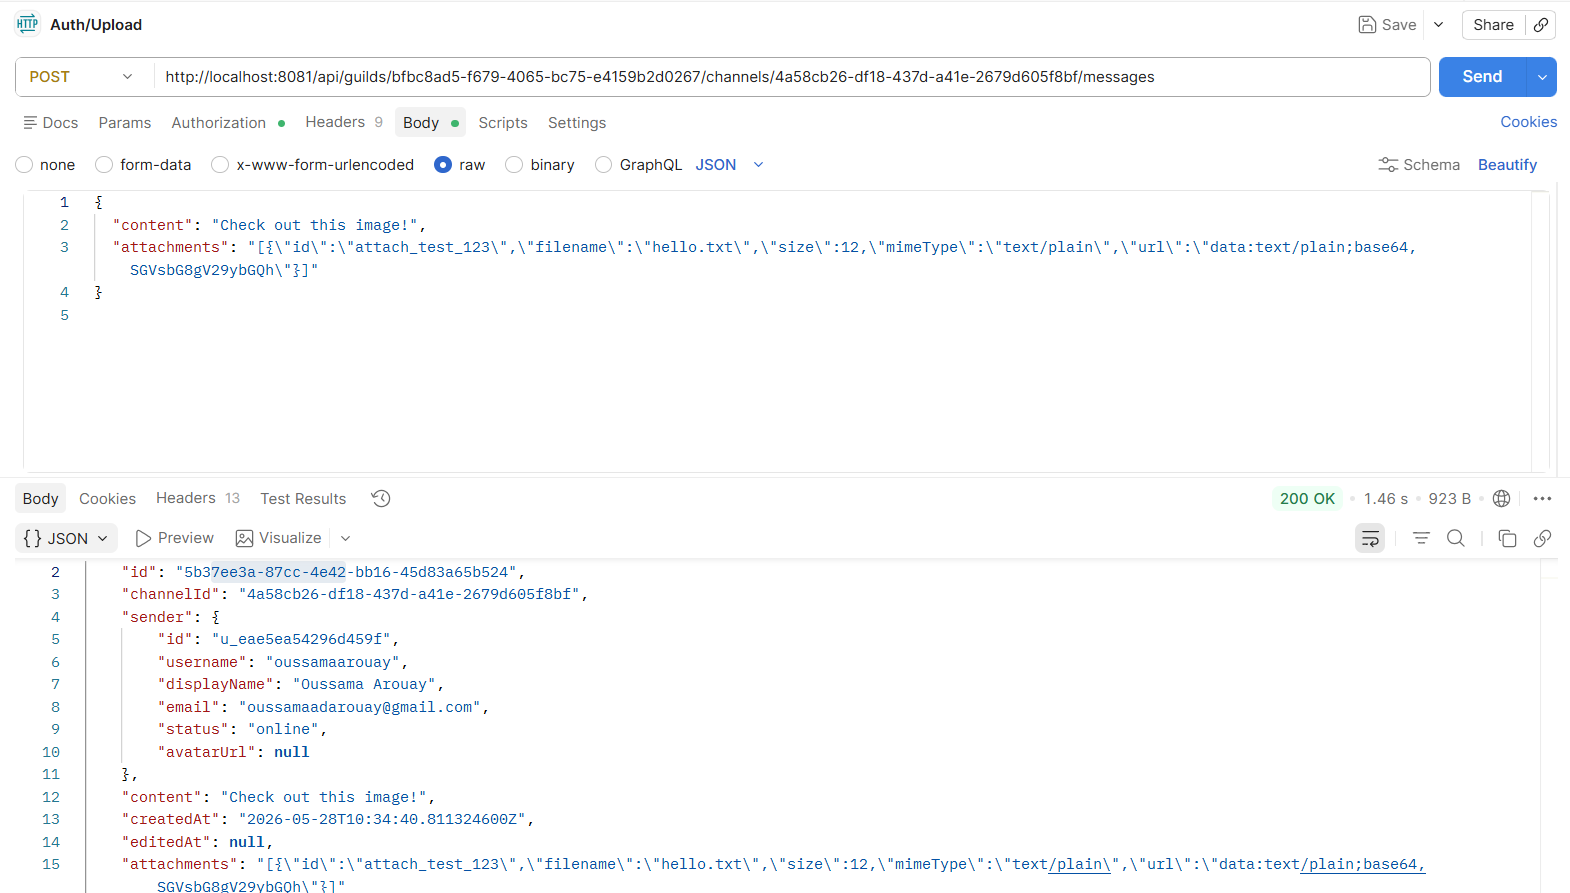
\includegraphics[width=0.7\textwidth]{upload file in channel.png}
    \caption{Audit: Uploading a File in a Channel.}
    \label{fig:sprint5_review_upload}
\end{figure}

\begin{figure}[H]
    \centering
    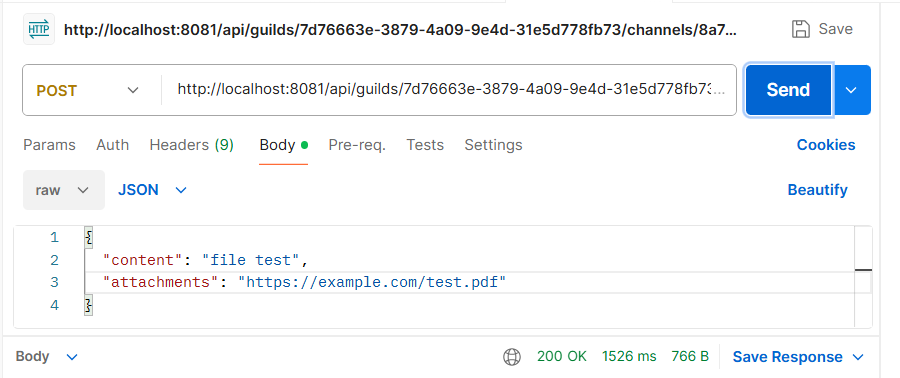
\includegraphics[width=0.7\textwidth]{file upload pdf.png}
    \caption{Audit: PDF File Upload Validation.}
    \label{fig:sprint5_review_pdf}
\end{figure}


\subsection{Sprint 5 Retrospective}
In this section, we discuss what we successfully accomplished as well as the missing elements of our sprint, presented in Table~\ref{tab:sprint5_retro}.

\renewcommand{\arraystretch}{1.5}
\begin{table}[H]
    \centering
    \begin{tabular}{| p{7.5cm} | p{7.5cm} |}
        \hline
        \textbf{Successes} & \textbf{Missing Elements} \\
        \hline
        \begin{itemize}
            \item Documented self-hosting options via Docker to protect communities against future data policy changes.
            \item Delivered file attachments for rich media sharing.
            \item Implemented dark mode theming for better user experience.
            \item Added direct message mention notifications.
            \item Validated security and access control for foundational server modules.
        \end{itemize} & 
        \begin{itemize}
            \item Failed to implement the screen sharing feature. WebRTC screen capture multiplexing alongside standard voice streams proved too technically complex for the timeframe.
        \end{itemize} \\
        \hline
    \end{tabular}
    \caption{Successes and missing elements of Sprint 5.}
    \label{tab:sprint5_retro}
\end{table}
\renewcommand{\arraystretch}{1.0}

\subsection{Graphical Design}
Graphical design, otherwise referred to as visual design, is an important part of visual product creation including websites, mobile apps, user interfaces, posters, logos, and ads.
In this section, we show mockup examples of our application to meet user requirements and improve user experience on a particular page.

The following figures showcase the visual design of the platform's key interfaces developed during Release 2.

\begin{itemize}
\item \textbf{Mockup «E2EE Text Messaging»}
\end{itemize}

\begin{figure}[H]
    \centering
    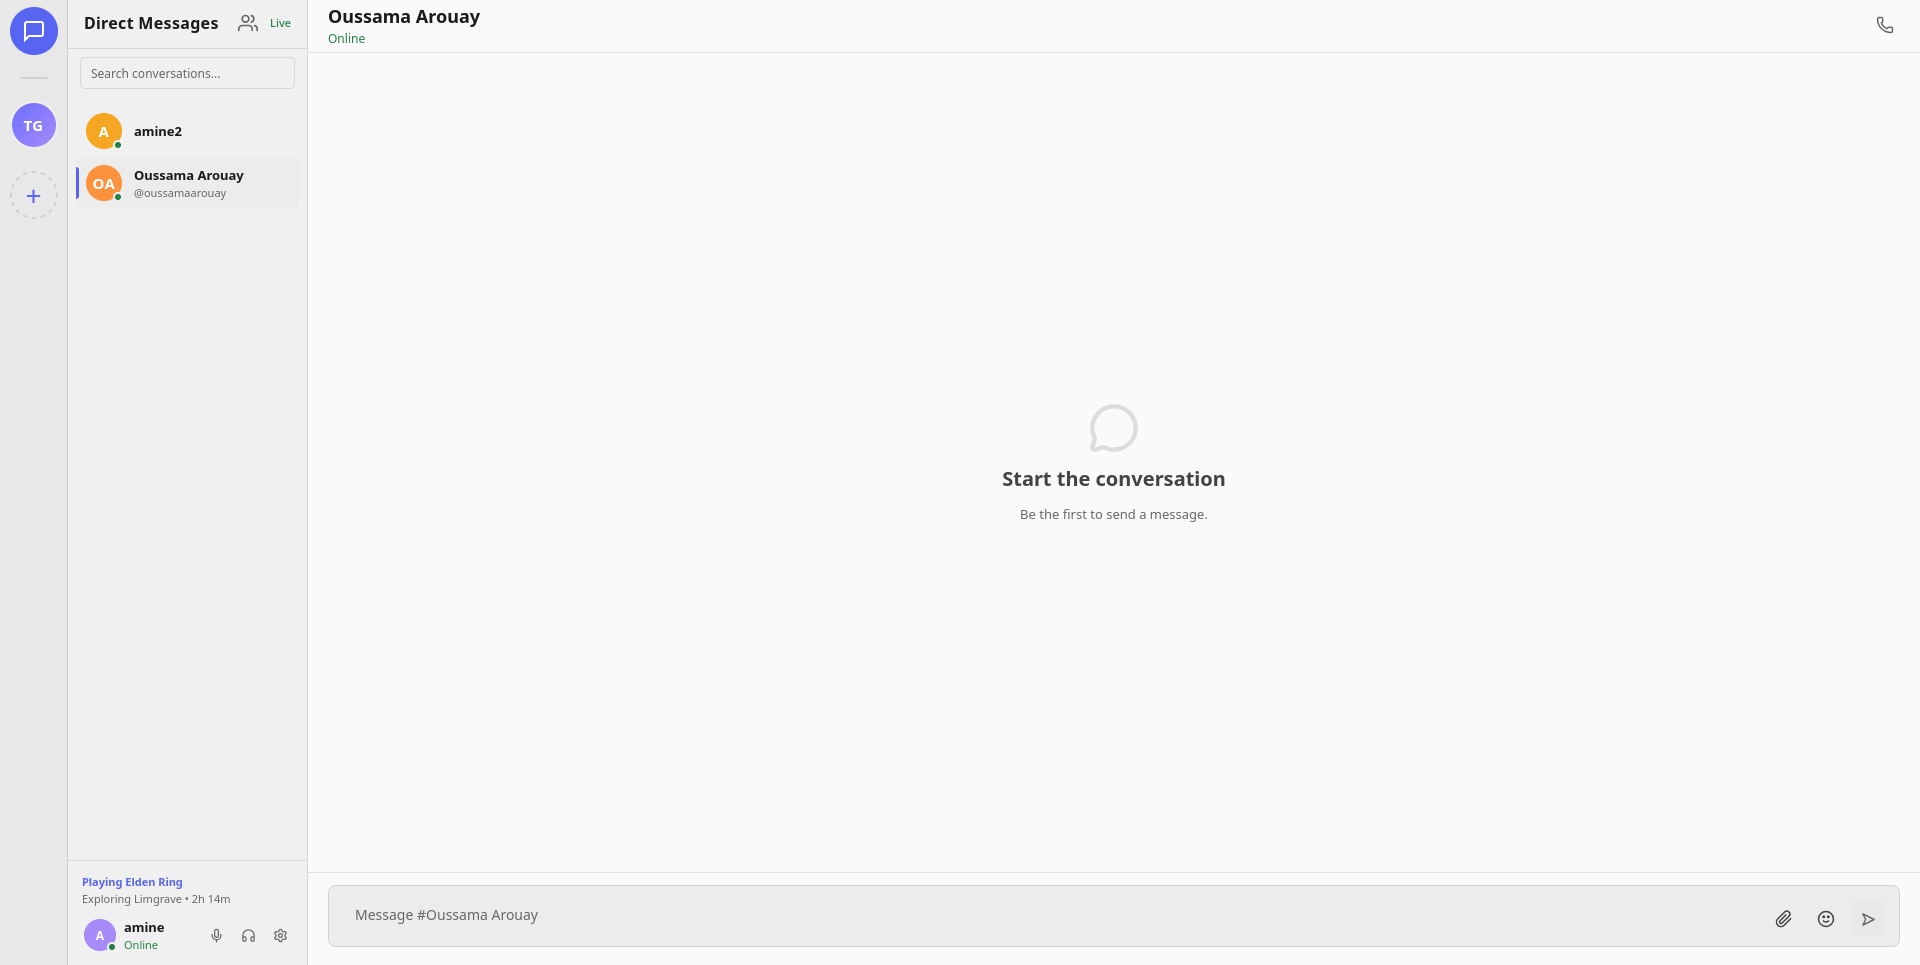
\includegraphics[width=0.7\textwidth]{new_conversation.png}
    \caption{Mockup: Initiating a New Conversation.}
    \label{fig:mock_new_conversation}
\end{figure}

\begin{figure}[H]
    \centering
    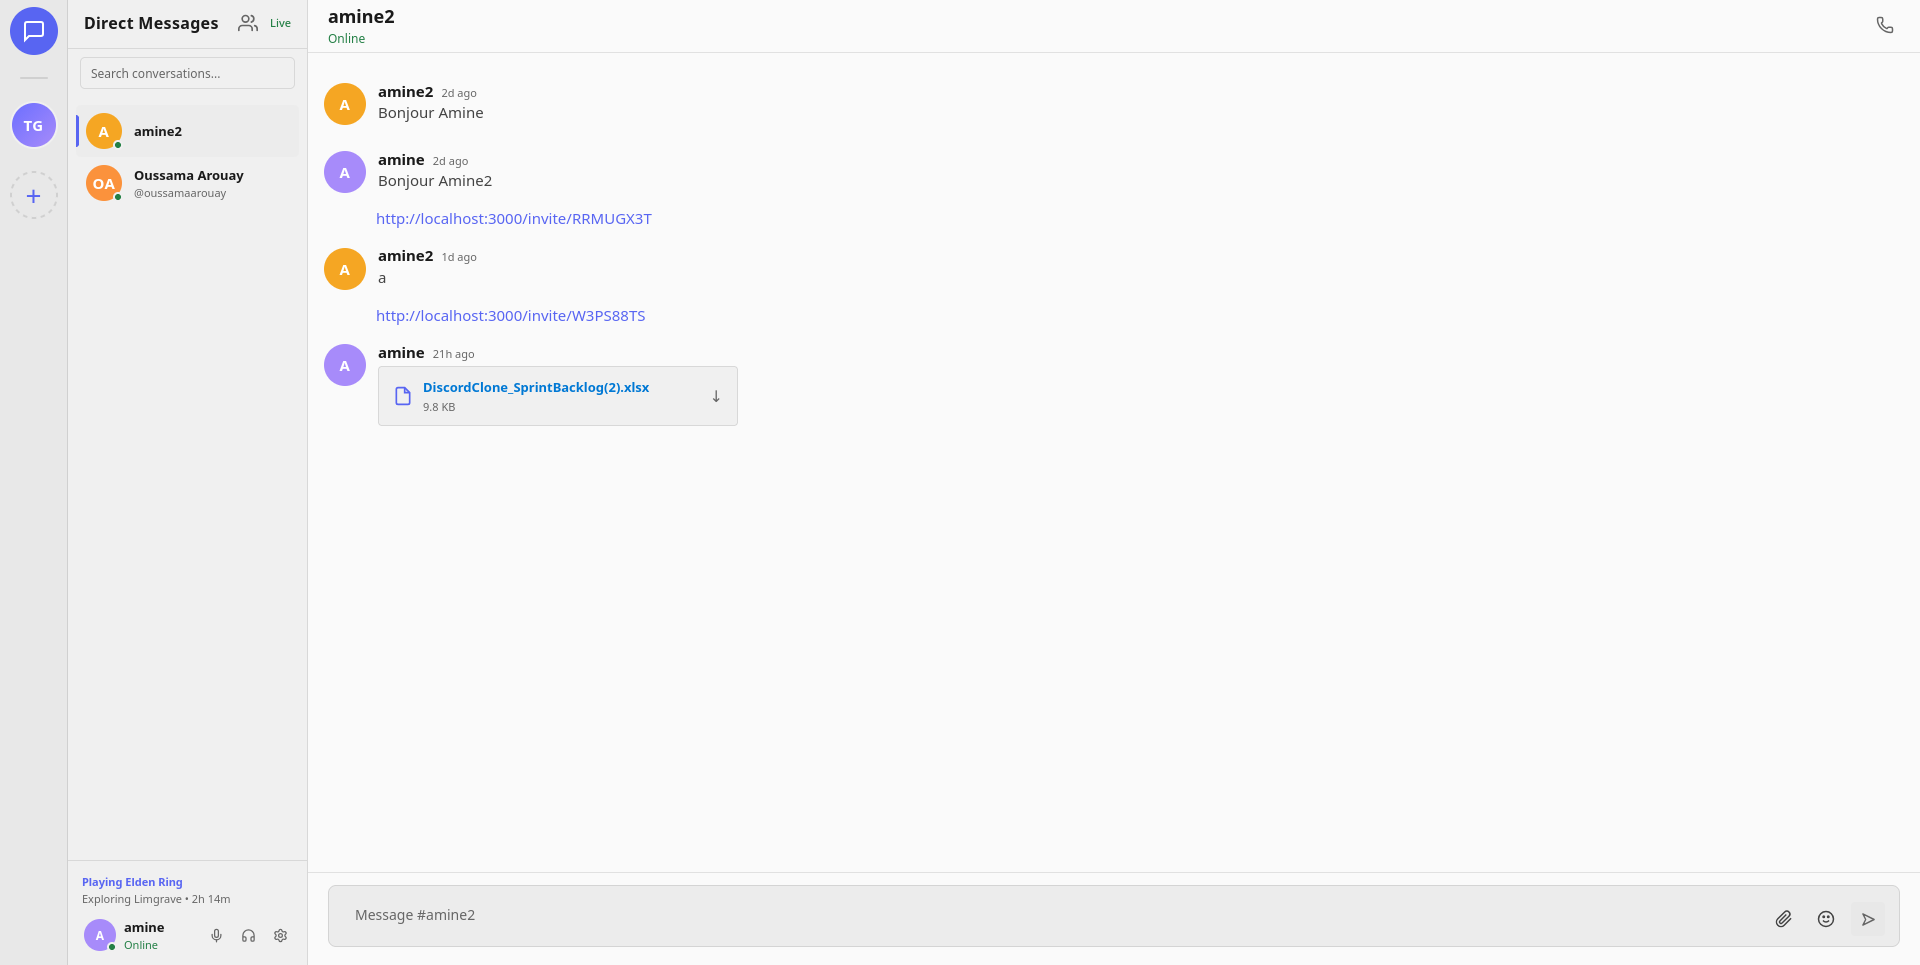
\includegraphics[width=0.7\textwidth]{old_conversation.png}
    \caption{Mockup: Viewing Conversation History.}
    \label{fig:mock_old_conversation}
\end{figure}

\begin{figure}[H]
    \centering
    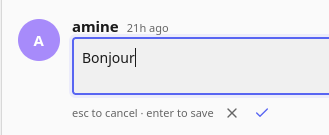
\includegraphics[width=0.7\textwidth]{message_edit.png}
    \caption{Mockup: Editing a Message.}
    \label{fig:mock_message_edit}
\end{figure}

\begin{figure}[H]
    \centering
    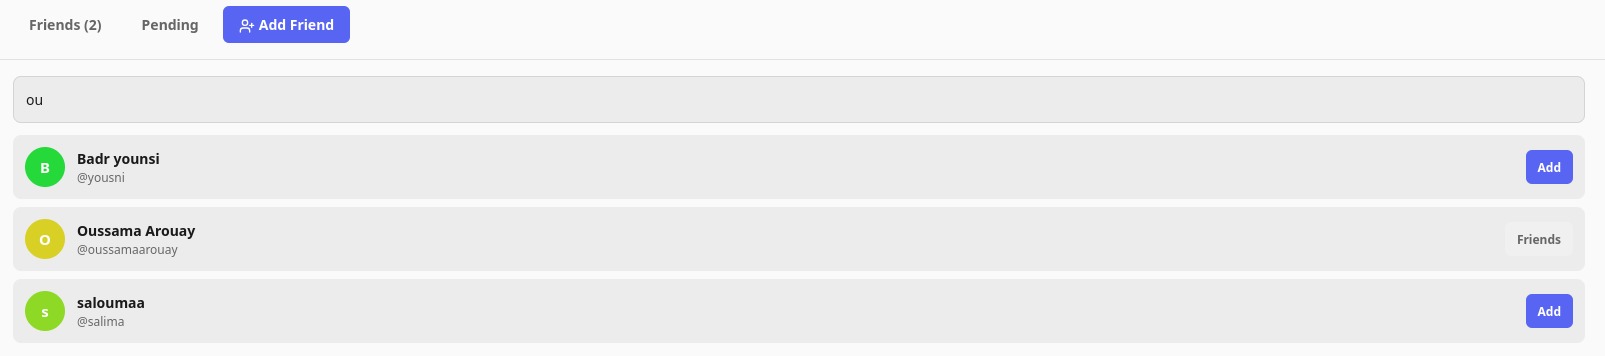
\includegraphics[width=0.7\textwidth]{friends_search.png}
    \caption{Mockup: Searching for Friends.}
    \label{fig:mock_friends_search}
\end{figure}

\begin{figure}[H]
    \centering
    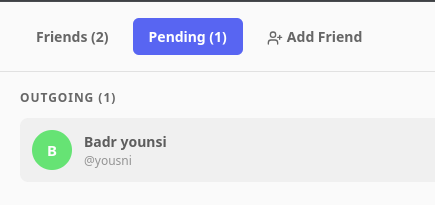
\includegraphics[width=0.7\textwidth]{pending_friend_request.png}
    \caption{Mockup: Handling a Pending Friend Request.}
    \label{fig:mock_pending_friend}
\end{figure}

\begin{itemize}
\item \textbf{Mockup «Secure Peer-to-Peer Voice Calls»}
\end{itemize}

\begin{figure}[H]
    \centering
    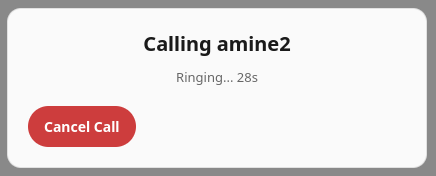
\includegraphics[width=0.7\textwidth]{ringing_user.png}
    \caption{Mockup: Incoming Voice Call (Ringing State).}
    \label{fig:mock_ringing_user}
\end{figure}

\begin{itemize}
\item \textbf{Mockup «Open-Source and Auditability (Extended)»}
\end{itemize}

\begin{figure}[H]
    \centering
    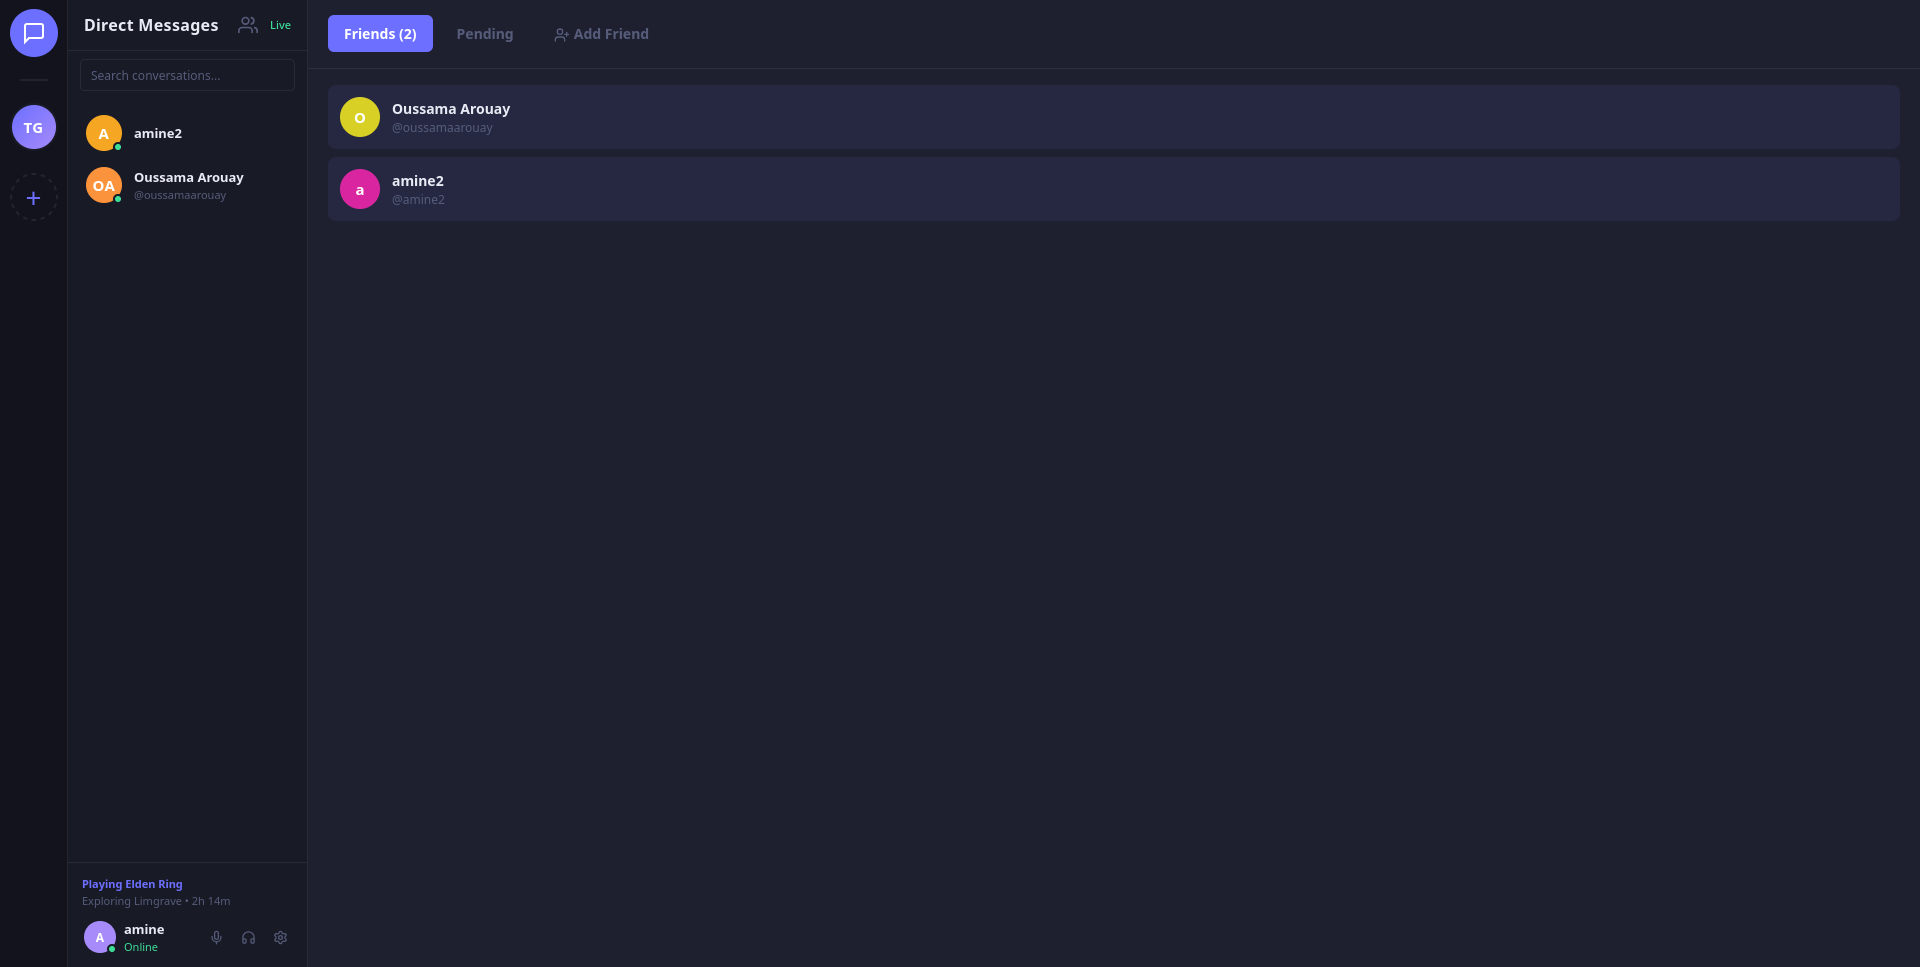
\includegraphics[width=0.7\textwidth]{landing_page_dark.png}
    \caption{Mockup: Landing Page (Dark Mode).}
    \label{fig:mock_landing_dark}
\end{figure}

\begin{figure}[H]
    \centering
    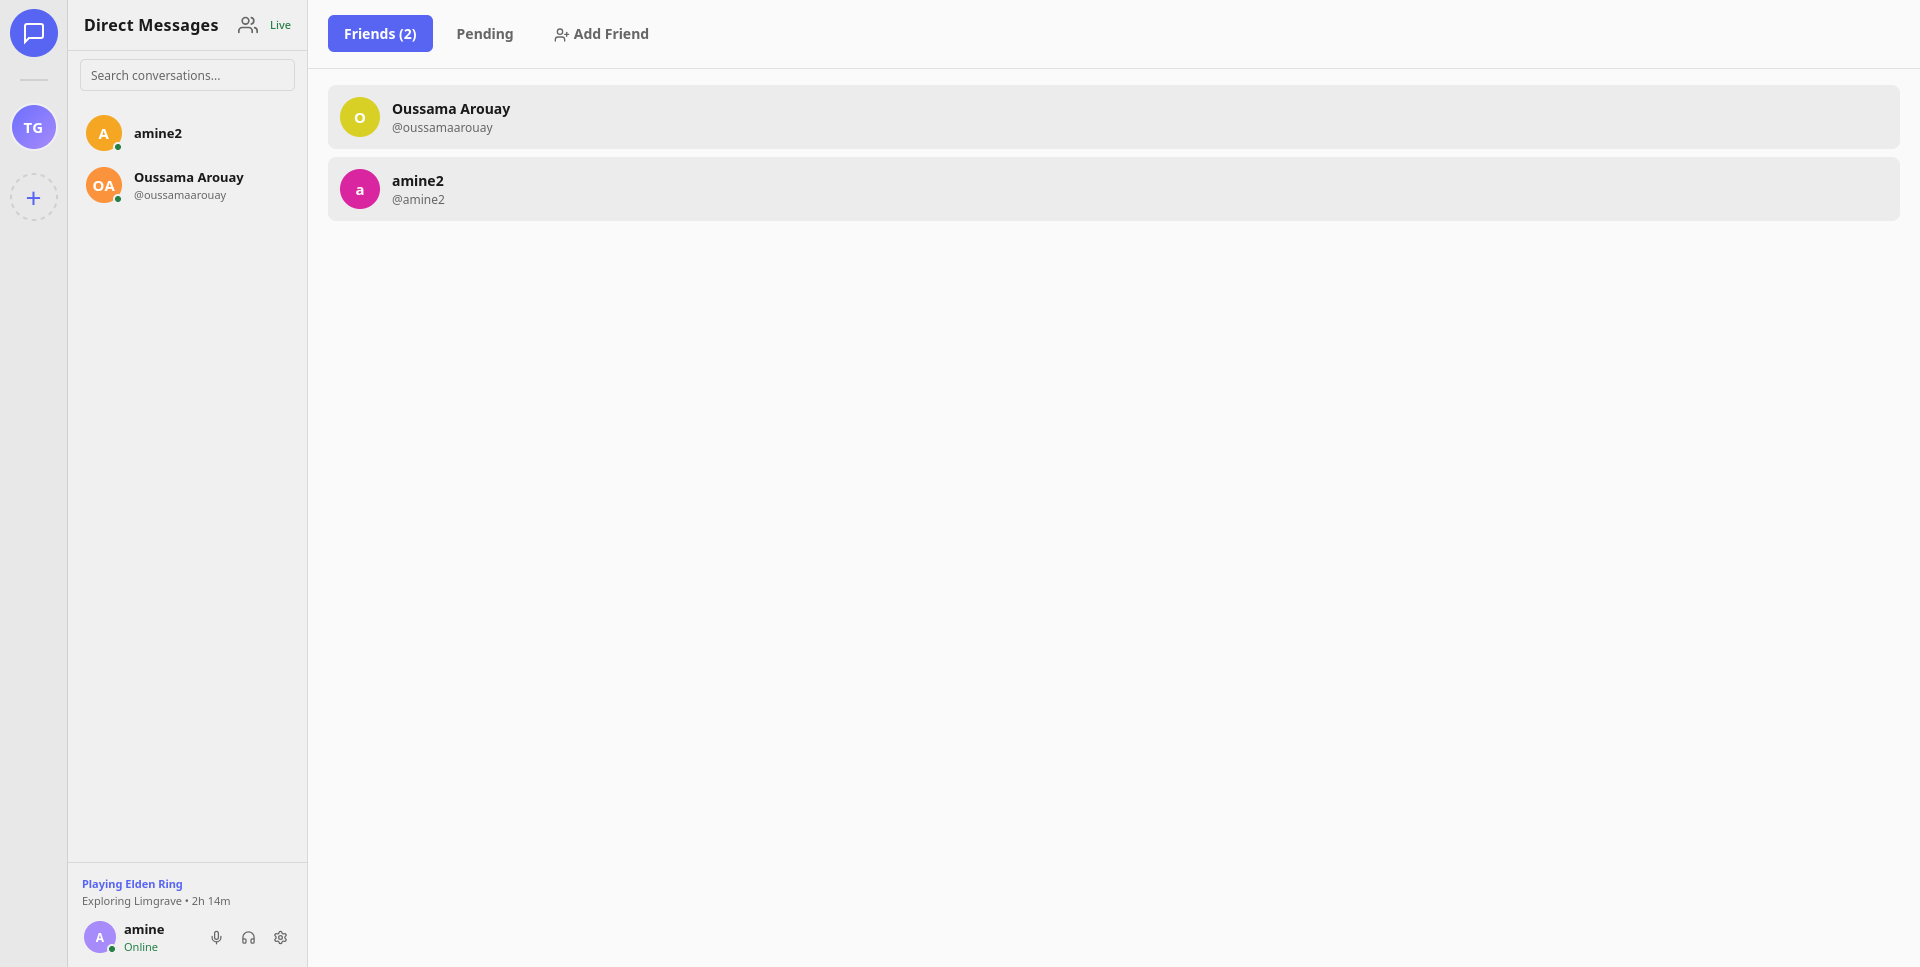
\includegraphics[width=0.7\textwidth]{landing_page_light.png}
    \caption{Mockup: Landing Page (Light Mode).}
    \label{fig:mock_landing_light}
\end{figure}


\begin{figure}[H]
    \centering
    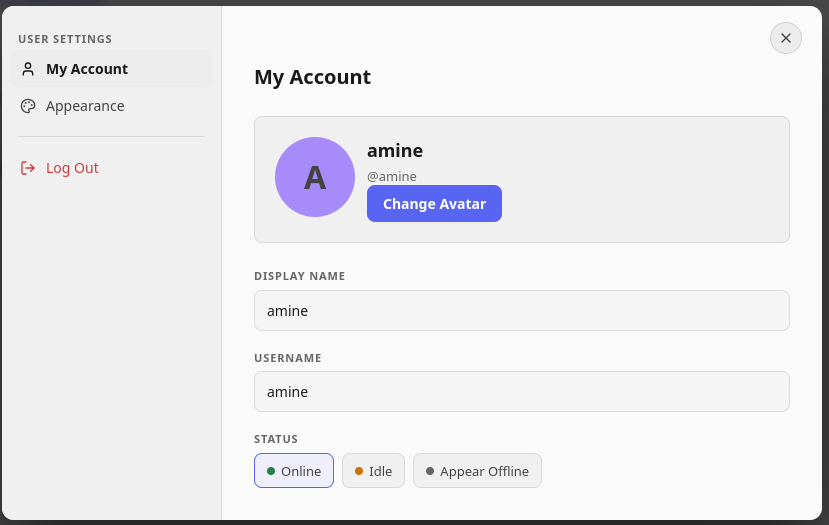
\includegraphics[width=0.7\textwidth]{user_settings.png}
    \caption{Mockup: User Account Settings.}
    \label{fig:mock_user_settings}
\end{figure}

\begin{figure}[H]
    \centering
    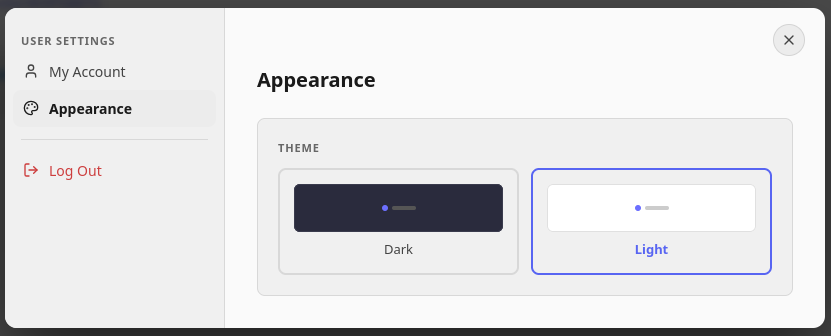
\includegraphics[width=0.7\textwidth]{appearance_settings.png}
    \caption{Mockup: Appearance and Theme Settings.}
    \label{fig:mock_appearance_settings}
\end{figure}

\begin{figure}[H]
    \centering
    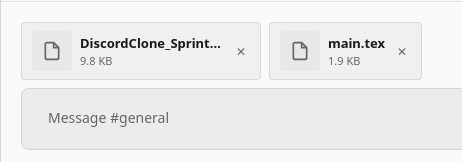
\includegraphics[width=0.7\textwidth]{files_attached.png}
    \caption{Mockup: File Attachment Interface.}
    \label{fig:mock_files_attached}
\end{figure}

\section{Conclusion}
This chapter detailed Release 2 of our secure alternative. By implementing E2EE text messaging in Sprint 3, secure WebRTC P2P audio channels in Sprint 4, and Docker self-hosting setups plus extended UI features in Sprint 5, we completed a robust privacy-first community communication system.